\documentclass{beamer}
\usetheme[progressbar=frametitle,block=fill]{metropolis}           % Use metropolis theme

\usepackage[spanish]{babel}
\usepackage[utf8]{inputenc}
\uselanguage{spanish}
\languagepath{spanish}
\deftranslation[to=spanish]{Theorem}{Teorema}
\deftranslation[to=spanish]{theorem}{teorema}

\usepackage{tikz}


\title{Pruebas de Conocimiento Cero y sus Aplicaciones}
\date{\today}
\author{José Luis Cánovas Sánchez\\[3mm]\scriptsize Tutores:\\Antonio José Pallarés Ruiz\\Leandro Marín Muñoz}

\institute{Universidad de Murcia\\Facultad de Matemáticas}



% La exposición durará entre 10 y 20 minutos y será en español, salvo 5 minutos que se expondrán en el idioma usado en el resumen de la memoria.


\begin{document}
\maketitle

\begin{frame}
	\frametitle{Outline}
	\tableofcontents
\end{frame}

\section{Decision Problems}

\begin{frame}{Decision Problem}
	\begin{block}{Definition (Decision Problem)}
		General description of a task which depend on some parameters and which possible answers are in the set $\{True, False \}$.
	\end{block}
	\begin{description}[Parameters]
		\item[Name] \textit{A characteristic name.}
		\item[Parameters] \textit{Arguments the problem depends on}.
		\item[Question] \textit{Question such the possible answers are} $True$ \textit{or} $False$.
	\end{description}
\end{frame}

\begin{frame}{Graph Isomorphism}
	\begin{description}[Parameters]
		\item[Name] Graph Isomorphism Problem (GI).
		\item[Parameters] Given two graphs $G_1 = (V_1, E_1)$ and $G_2 = (V_2, E_2)$ with $\mid V_1 \mid = \mid V_2 \mid = n$.
		\item[Question] Is there an isomorphism $\tau : V_1 \rightarrow V_2$ such that an edge $(u,v)\in E_1$ if and only if $(\tau (u),\tau (v)) \in E_2$?
	\end{description}



		
	\begin{center}
		% Define style for nodes
	\tikzstyle{every node}=[circle, draw, fill=black!50, inner sep=0pt, minimum width=4pt]
	%  Tutte's 8-cage
	\begin{tikzpicture}[thick,scale=0.5]
	% The following path utilizes several useful tricks and features:
	% 1) The foreach statement is put inside a path, so all the edges
	%    will in fact be a the same path.
	% 2) The node construct is used to draw the nodes. Nodes are special
	%    in the way that they are drawn *after* the path is drawn. This
	%    is very useful in this case because the nodes will be drawn on
	%    top of the path and therefore hide all edge joins.
	% 3) Simple arithmetics can be used when specifying coordinates.
	\draw \foreach \x in {0,36,...,324}
	{
		(\x:2) node {}  -- (\x+108:2)
		(\x-10:3) node {} -- (\x+5:4)
		(\x-10:3) -- (\x+36:2)
		(\x-10:3) --(\x+170:3)
		(\x+5:4) node {} -- (\x+41:4)
	};
	\end{tikzpicture}\quad
	\begin{tikzpicture}[thick,scale=0.5]
	\draw \foreach \x in {0,36,...,324}
	{
		(\x:2.5) node {}  -- (\x+108:2.5)
		(\x-10:4) node {} -- (\x+5:1)
		(\x-10:4) -- (\x+36:2.5)
		(\x-10:4) --(\x+170:4)
		(\x+5:1) node {} -- (\x+41:1)
	};
	\end{tikzpicture}
	\end{center}
\end{frame}


\begin{frame}{Complexity classes}

\begin{block}{Definition (Class P)}
	The set of decision problems which can be solved in polynomial time.
\end{block}

\begin{block}{Definition (Class NP)}
	The set of decision problems where a $True$ answer can be verified in polynomial time, given some extra information (certificate).
\end{block}

\begin{block}{Fact}
	$P\subset NP$
\end{block}

\begin{block}{Millennium Problem}
	$P\overset{?}{=} NP$ % P versus NP
\end{block}


\end{frame}






\section{Quadratic Residues}

\begin{frame}{Quadratic Residues}
\begin{definition}
	Given $x\in \mathbb{Z}^*_n$ we say that $x$ is a \textit{quadratic residue}
	modulo $n$ if there exists an $a \in \mathbb{Z}^*_n$ such thtat
	
	$x \equiv a^2 \, mod \, n$.
	
	If said $a$ doesn't exist, then $x$ is called a \textit{quadratic non-residue}.
\end{definition}

We define $Q_n$ as the set of quadratic residues modulo $n$, and $\overline{Q_n}$ the set of quadratic non-residues.
\end{frame}



%\section{Residuos Cuadráticos}
%
%\begin{frame}{Residuos Cuadráticos}
%	\begin{definition}
%		Sea $x\in \mathbb{Z}^*_n$. Se dice que $x$ es un \textit{residuo cuadrático}
%		módulo n, o un \textit{cuadrado} módulo n, si existe un $a \in \mathbb{Z}^*_n$
%		tal que
%		
%		$x \equiv a^2 \, mod \, n$.
%		
%		Si no existe dicho $a$, entonces $x$ se llama un \textit{no-residuo cuadrático} módulo n.
%	\end{definition}
%
%	Al conjunto de los residuos cuadráticos módulo n los denotaremos como $Q_n$.
%	Al de los no-residuos cuadráticos, como $\overline{Q_n}$.
%\end{frame}



%\begin{frame}{Quadratic Residues}
%\begin{block}{Example}
%	If we take $n=4$, the quadratic non-residues are $2$ and $3$, and the only quadratic residue is $1$:
%	\begin{align*}
%	1^2 \equiv 1 \, mod \, 4 \qquad 2^2 \equiv 0 \, mod \, 4 \qquad  3^2 \equiv 1 \, mod \, 4
%	\end{align*}
%\end{block}
%\textbf{Note:} By definition  $0 \notin \mathbb{Z}^*_n$, therefore $0 \notin Q_n$ and $0 \notin \overline{Q_n}$.
%\end{frame}

%\begin{frame}{Residuos Cuadráticos}
%	\begin{example}
%		Si tomamos $n=4$, los no-residuos cuadráticos son $2$ y $3$, y el único residuo cuadrático es $1$:
%		\begin{align*}
%		1^2 \equiv 1 \, mod \, 4 \qquad 2^2 \equiv 0 \, mod \, 4 \qquad  3^2 \equiv 1 \, mod \, 4
%		\end{align*}
%	\end{example}
%	Por definición $0 \notin \mathbb{Z}^*_n$, y por tanto $0 \notin Q_n$ ni $0 \notin \overline{Q_n}$.
%\end{frame}

\begin{frame}{Quadratic Residues: Legendre Symbol}
\begin{definition}[Legendre Symbol]
	Given an odd primes $p$ and an integer $a$, we define the \textit{Legendre Symbol} as:
	
	\begin{center}
		$
		\left( \dfrac{a}{p} \right) =
		\begin{cases}
		0, & if\ a \equiv 0 \, mod \, p\\
		1, & if\ a \in Q_p  \\
		-1, & if\ a \in \overline{Q_p} \\
		\end{cases}
		$
	\end{center}
\end{definition}
\end{frame}


%\begin{frame}{Residuos Cuadráticos: Símbolo de Legendre}
%	\begin{definition}[Símbolo de Legendre]
%		Dados un primo impar $p$ y un entero $a$, se define el {\em Símbolo de Legendre} como
%		
%		\begin{center}
%			$
%			\left( \dfrac{a}{p} \right) =
%			\begin{cases}
%			0, & si\ a \equiv 0 \, mod \, p\\
%			1, & si\ a \in Q_p  \\
%			-1, & si\ a \in \overline{Q_p} \\
%			\end{cases}
%			$
%		\end{center}
%	\end{definition}
%\end{frame}


\begin{frame}{Quadratic Residues: Jacobi Symbol}
\begin{definition}[Jacobi Symbol]
	Be $n$ is an odd integer with prime factorization $n = p_1^{e_1} p_2^{e_2} \cdots p_r^{e_r}$, and $a$ an integer. Then we define the \textit{Jacobi Symbol} of $a$ as:
	\[\left( \dfrac{a}{n} \right) = \left( \dfrac{a}{p_1} \right)^{e_1} \cdot \left( \dfrac{a}{p_2} \right)^{e_2} \cdot \cdots \cdot \left( \dfrac{a}{p_t} \right)^{e_t}\]
\end{definition}
\end{frame}

%\begin{frame}{Residuos Cuadráticos: Símbolo de Jacobi}
%	\begin{definition}[Símbolo de Jacobi]
%		Sea $n$ un entero impar positivo cuya descomposici\'on en factores primos es $n = p_1^{e_1} p_2^{e_2} \cdots p_r^{e_r}$ y sea $a$ un entero. Entonces definimos
%		el \textit{s\'imbolo de Jacobi} de $a$ y $n$ como
%		\[\left( \dfrac{a}{n} \right) = \left( \dfrac{a}{p_1} \right)^{e_1} \cdot \left( \dfrac{a}{p_2} \right)^{e_2} \cdot \cdots \cdot \left( \dfrac{a}{p_t} \right)^{e_t}\]
%	\end{definition}
%\end{frame}


\begin{frame}{Quadratic Residues: Properties}
\begin{itemize}
	\item Using the \textbf{Chinese Remainder Theorem} it is equivalent to work with quadratic residues in ${\mathbb Z}_{pq}$ or in ${\mathbb Z}_p$ and ${\mathbb Z}_q$.
	\item We can compute a \textbf{square root} modulo a \textbf{prime} in polynomial time with \textbf{Tonelli Algorithm}.
	\item \textbf{Jacobi} Symbol can be computed in polynomial time \textbf{without} the module factorization.
	\item \textbf{Jacobi} Symbol $1$ does not imply a \textit{quadratic residue}.
	\item Given a module \textbf{factorization}, we can compute the modular \textbf{square roots} in polynomial time with the \textit{Chinese Remainder Theorem} and \textit{Tonelli} Algorithm.
\end{itemize}
\end{frame}

%\begin{frame}{Quadratic Residues: Properties}
%\begin{itemize}
%	\item Given a prime $p$, $|Q_p| = |\overline{Q_p}| = \frac{p-1}{2}$.
%	\item Given $n$, $m$ coprime,  $x \in {\mathbb Z}_{mn}$ is a quadratic residue if and only if $x~mod~m$ and   $x~mod~n$ are respectively quadratic residues in ${\mathbb Z}_m$ and ${\mathbb Z}_n$.
%	\item If $a$ and $b$ are square roots of $x~mod~m$ and $x~mod~n$, we can use the \textbf{Chinese Remainder Theorem} to combine both as a square root of $x$ in ${\mathbb Z}_{mn}$.
%	\item Be $n = pq$, $p$ and $q$ different primes, then $|Q_n| = \frac{(p-1)(q-1)}{4}$
%\end{itemize}
%\end{frame}


%\begin{frame}{Residuos Cuadráticos: Propiedades}
%	\begin{itemize}
%		\item Sea $p>1$ un n\'umero primo, entonces $|Q_p| = |\overline{Q_p}| = \frac{p-1}{2}$.
%		\item Sean $n$, $m$ coprimos. $x \in {\mathbb Z}_{mn}$ es un residuo cuadr\'atico si y s\'olo si $x~mod~m$
%		y $x~mod~n$ son residuos cuadr\'aticos en ${\mathbb Z}_m$ y ${\mathbb Z}_n$
%		respectivamente.
%		\item Si $a$ y $b$ son ra\'ices cuadradas de $x~mod~m$ y $x~mod~n$ en sus
%		correspondientes anillos, podemos combinarlas mediante el \textbf{Teorema Chino de los Restos}
%		para obtener una ra\'iz cuadrada de $x$ en ${\mathbb Z}_{mn}$.
%		\item Sea $n = pq$ el producto de dos primos distintos, entonces el n\'umero de residuos cuadr\'aticos m\'odulo $n$ es $\frac{(p-1)(q-1)}{4}$.
%	\end{itemize}
%\end{frame}

%\begin{frame}{Quadratic Residues: Properties}
%\begin{itemize}
%	\item We can compute a \textbf{square root} modulo a prime in polynomial time with \textbf{Tonelli Algorithm}.
%	\item \textbf{Jacobi} Symbol can be computed in polynomial time \textbf{without} the module factorization.
%	\item \textbf{Jacobi} Symbol $1$ does not imply a \textit{quadratic residue}.
%	\item Given a module \textbf{factorization}, we can compute the modular \textbf{square roots} in polynomial time with the \textit{Chinese Remainder Theorem} and \textit{Tonelli} Algorithm.
%\end{itemize}
%\end{frame}

%\begin{frame}{Residuos Cuadráticos}
%	\begin{itemize}
%		\item El Símbolo de \textbf{Legendre} nos indica si un entero es residuo cuadrático módulo un \textbf{primo} mayor que 2.
%		\item Podemos calcular una \textbf{raíz} cuadrada módulo un primo en tiempo polinomial con el \textbf{Algoritmo de Tonelli}.
%		\item El Símbolo de \textbf{Jacobi} se puede calcular en tiempo polinomial \textbf{sin} conocer la \textbf{factorización} del módulo.
%		\item Un Símbolo de \textbf{Jacobi} $-1$ nos indica \textit{no-residuo}, pero un $1$ ya no indica necesariamente \textit{residuo cuadrático}.
%		\item Conociendo la \textbf{factorización} del módulo, podemos calcular la \textbf{raíz} modular en tiempo \textbf{polinomial} con el \textbf{Teorema Chino de los Restos} y el \textbf{Algoritmo de Tonelli}.
%	\end{itemize}
%\end{frame}

\begin{frame}{Quadratic Residues: QR Problem}
	\begin{description}[Parameters]
		\item[Name] Quadratic residue problem (QR).
		\item[Parameters] Given a composite integer $N=pq$ and the integer $x$ with Jacobi Symbol $\left( \frac{x}{N} \right) = 1$.
		\item[Question] Is $x$ a quadratic residue in ${\mathbb Z}_N$? $\exists a\in {\mathbb Z}_N : x\equiv a^2 (N)$?
	\end{description}
\end{frame}

%\begin{frame}{Residuos Cuadráticos: Problema QR}
%	\begin{description}[Parámetros]
%		\item[Nombre] Problema de los residuos cuadr\'aticos (QR).
%		\item[Parámetros] $N$ un entero impar tal que $N = pq$ para $p$ y $q$ primos, y el entero $x$ tal que $\left( \frac{x}{N} \right) = 1$.
%		\item[Pregunta] ¿Es $x$ un residuo cuadrático en ${\mathbb Z}_N^*$?
%	\end{description}
%\end{frame}


\section{Pruebas Interactivas}

\begin{frame}{Pruebas Interactivas}
	
	\begin{description}[Verificador (V)]
		\item[Probador (P)] computacionalmente \textit{todopoderosa}.
		\item[Verificador (V)] cómputo limitado, probabilístico de tiempo de polinomial.	
	\end{description}
	{\Large\[P \leftrightarrows  V\]}
	\textbf{Objetivo:} P quiere probar \textit{algo} a V, p. ej., que una instancia de un problema es $Verdadera$.

\end{frame}

\begin{frame}{Pruebas Interactivas}
	\begin{definition}[Sistema de Prueba Interactiva]
		
		Un problema de decisión $Q$ tiene un \textit{sistema de prueba interactiva} si tiene un protocolo de interacción polinomialmente acotado en número de mensajes que cumple:
		
		\begin{itemize}
			\item \textit{Completitud} Para toda instancia $q$ $Verdadera$, del problema $Q$, V acepta $q$ como $Verdadera$.
			\item \textit{Robustez} Para cada instancia $q$ $Falsa$, V rechaza la prueba de $q$ con una probabilidad no menor que $\epsilon = 1-n^{-c}$, para cualquier constante $c>0$ y donde $n$ es el tamaño de la instancia.
		\end{itemize}
		
	\end{definition}
\end{frame}

\begin{frame}{Ejemplo Pruebas Interactivas: Problema QR}
	\begin{theorem}
		El problema QR tiene un sistema de prueba interactivo.
	\end{theorem}

	\begin{description}[Parámetros]
		\item[Nombre] Problema de los residuos cuadr\'aticos (QR).
		\item[Parámetros] $N$ un entero impar tal que $N = pq$ para $p$ y $q$ primos, y el entero $x$ tal que $\left( \frac{x}{N} \right) = 1$.
		\item[Pregunta] ¿Es $x$ un residuo cuadrático en ${\mathbb Z}_N^*$?
	\end{description}
\end{frame}


\begin{frame}{Ejemplo Pruebas Interactivas: Problema QR}
\begin{block}{Prueba interactiva para QR $(x,N)$}
	
	Sea $t(n)$ un polinomio en $n$, el tamaño de la instancia $(x,N)$. P y V repiten $t(n)$ veces los siguientes pasos.
	
	\begin{enumerate}
		
		\item P $\rightarrow$ V :\quad $u \in_R \mathbb{Z}^{Q+}_N$, \; un residuo cuadrático en $\mathbb{Z}_N$.
		
		\item V $\rightarrow$ P :\quad $b \in_R \{0,\,1\}$.
		
		\item P $\rightarrow$ V :\quad $w$,\; una raíz cuadrada aleatoria de $u\cdot x^b$.
		
		\item V comprueba si:
		\[
		w^2 \overset{?}{\equiv}
		\begin{cases}
		u\, mod\, N, & si\ b = 0\\
		xu\, mod\, N, & si\ b = 1.\\
		\end{cases}
		\]
		
		Si la comparación falla, V termina en rechazo. En caso contrario, vuelve al paso 1.
		
	\end{enumerate}
	
\end{block}
\end{frame}


\begin{frame}{Ejemplo Pruebas Interactivas: Problema QR}
	\begin{proof}
		La prueba es \textbf{completa}:
		
		Instancia $(x,N)$ $Verdadera$ $\Rightarrow$ $x$ es residuo cuadrático, existe raíz.
		
		P computacionalmente todopoderoso $\Rightarrow$ puede calcular $w$ raíz de $u$ o $xu$, residuos cuadráticos.
		
		V acepta la prueba de P.
	\end{proof}
\end{frame}

\begin{frame}{Ejemplo Pruebas Interactivas: Problema QR}
\begin{proof}
	La prueba es \textbf{robusta}:
	
	Instancia $Falsa$, $x$ no residuo cuadrático.
	P$^*$ intenta adivinar el reto $b\in_R\{0,1\}$.
	\begin{itemize}
		\item Si $b=0$, sigue el protocolo, elige $u \in_R \mathbb{Z}^{Q+}_N$.
		
		\item Si $b=1$, elige $u \equiv x^{-1} a^2 \, mod \, N$, con $a \in_R \mathbb{Z}_N$.
		Responde con $w = a$.		
		V comprobará $w^2\equiv a^2 \overset{?}{\equiv} x\cdot x^{-1} a^2 \equiv a^2 \, mod \, N$.
	\end{itemize}

	Si P$^*$ falla al adivinar, o no existirá raíz de $xu$, o $w^2 \not \equiv u \, mod \, N$.
	
	Probabilidad de acertar el reto $b$: $\frac{1}{2}$.
	
	Probabilidad de pasar la prueba: $2^{-t(n)}$.
	
\end{proof}
\end{frame}



\section{Pruebas de Conocimiento Cero}


\begin{frame}{Pruebas de Conocimiento Cero} 
	\begin{definition}[Ensamble] 
		Llamamos ensamble probabilístico (\textit{ensemble} en inglés) a una familia de variables aleatorias $\{X_i\}_{i\in I}$, con $I$ numerable. 
	\end{definition} 
	$ Vista_{P,V^*}(q,h) = (q,\,h,\,A_1,\,B_1,\,C_1, \dots ,\,A_{t(n)},\,B_{t(n)},\,C_{t(n)}). $ 
	
	\begin{definition}[Simulador] 
		Un Simulador $S_{V^*}(q,h)$ es un algoritmo probabilístico de tiempo polinomial, que utiliza toda la información que V$^*$ tiene disponible, para generar una transcripción de una prueba interactiva, para una instancia $q$ del problema $Q$, sin necesidad de interactuar con P. 
	\end{definition} 
	Si V no sigue el protocolo, elegirá los retos en base a un algoritmo $F(\cdot)$ en base a toda la información disponible. 
\end{frame} 


\begin{frame}{Pruebas de Conocimiento Cero}
	\begin{definition}[Propiedad de conocimiento cero]
		Un sistema de prueba interactiva (completo y robusto), para un problema de decisión $Q$, es de \textit{conocimiento cero} si el ensamble $Vista_{P,V}(q,h)$ es idéntico al ensamble generado por un Simulador $S_{V^*}(q,h)$, para cualquier instancia $Verdadera$ $q\in Q$ y cualquier historial $h$.
	\end{definition}

	Toda la información que se pueda obtener de interactuar con P, se puede obtener sin interactuar con P.
\end{frame}



\begin{frame}{Pruebas de Conocimiento Cero: Problema QR}
	\begin{theorem}
		La prueba interactiva del problema QR es de conocimiento cero.
	\end{theorem}
	\textbf{Demostración}
	
	\textbf{Variables aleatorias}
	\begin{description}[Wi]
		\item[$U_i$] El residuo cuadrático aleatorio enviado por P en el primer mensaje, $u \in_R \mathbb{Z}^{Q+}_N$.
		
		\item[$B_i$] El reto aleatorio generado por V, $b \in_R \{0,\,1\}$.
		
		\item[$W_i$] La \textit{prueba} de P, $w \in_R \Omega_u$ o bien $w \in_R \Omega_{xu}$.
	\end{description}

	\[  Vista_{P,V^*}(x,N,h) = (x,N,h,U_1,B_1,W_1,\dots , U_{t(n)}, B_{t(n)}, W_{t(n)}) \]
\end{frame}

\begin{frame}{Pruebas de Conocimiento Cero: Problema QR}
	\textbf{Probabilidad en la Vista}
	\[
	P(U_i=u, B_i=b, W_i=w) = 
	\]
	\[ P(U_i=u)\cdot P(B_i=b \mid U_i=u) \cdot P(W_i=w \mid U_i=u, B_i=b) \]
	
	Sea $\alpha = \mid \mathbb{Z}^{Q+}_N \mid $, entonces $P(U_i=u) = \frac{1}{\alpha}$.
	
	Denotamos $ P(B_i=b \mid U_i=u)=p_b$, dependerá de $F$.
	
	Por último, sea $\beta = \mid \Omega_u \mid = \mid \Omega_{xu} \mid $. $u$ fijo por construcción. Entonces:
	\[P(W_i=w \mid U_i=u, B_i=0) = 1/\beta,\ \forall w \in \Omega_u\]
	\[P(W_i=w \mid U_i=u, B_i=1) = 1/\beta,\ \forall w \in \Omega_{xu}\]
	
	En total nos queda, $P(U_i=u, B_i=b, W_i=w) = \frac{p_b}{\alpha \beta}$.
\end{frame}

\begin{frame}{Pruebas de Conocimiento Cero: Problema QR}
	\textbf{Simulador} Instancia $(x,N)$ $Verdadera$ del problema QR.\\
	\textit{Ejecución}: Generadas las primeras $i$ rondas. Repetir para $i+1 \leq t(n)$:
	
	\begin{enumerate}
		\item Elegir $b_{i+1} \in_R \{0,\,1\}$
		
		\item Elegir $w_{i+1} \in_R \mathbb{Z}^*_N$
		
		\item \textbf{Si} $b_{i+1} = 0$, \textbf{entonces} calcular \qquad $u_{i+1} \equiv w_{i+1}^2 \, mod \,  N$ \\
		\textbf{Si no}, \qquad \qquad \qquad \qquad \qquad \qquad \: $u_{i+1} \equiv w_{i+1}^2 \cdot x^{-1} \, mod \,  N$
		
		\item \textbf{Si} $b_{i+1} = F(x,N,h,v_i,u_{i+1})$, \textbf{entonces} añadir la tupla \\ $(u_{i+1},\,b_{i+1},\,w_{i+1})$ a la transcripción. \textbf{Si no}, volver al paso 1.
		
		\item $i = i+1$
		
	\end{enumerate}
\end{frame}


\begin{frame}{Pruebas de Conocimiento Cero: Problema QR}
	\textbf{Probabilidad del Simulador}
	{\small\[P(U_i=u, B_i=b, W_i=w) = \]
	\[P(W_i=w)\cdot P(B_i=b \mid U_i=u) \cdot P(U_i=u \mid W_i=w, B_i=b)\]}

	{\small Sabemos que $\mid \mathbb{Z}^*_N \mid = \alpha \cdot \beta $, por lo que $P(W_i=w) = \frac{1}{\alpha \beta}$.}
	{\tiny\begin{align*}
	P(U_i=u) &= \sum_{w\in \Omega_u} P(U_i=u, W_i=w, B_i = 0) + \sum_{w\in \Omega_{xu}} P(U_i=u, W_i=w, B_i = 1) =  \\
	&= \sum_{w\in \Omega_u} P(W_i=w)P(B_i = 0) + \sum_{w\in \Omega_{xu}} P(W_i=w)P(B_i = 1) = \\
	&=\beta \cdot \frac{1}{\alpha \beta} \cdot (P(B_i=0) + P(B_i=1)) = \frac{1}{\alpha}
	\end{align*}}
	{\small $\Rightarrow U_i$ misma distribución que $U_i$ de la $Vista$ $\Rightarrow$ $P(B_i=b \mid U_i=u) = p_b$, depende de $F(\cdot)$.}
	
	%Por construcción, dados $w$ y $b$ en el simulador, $u$ tiene un único valor posible, $u\equiv w^2x^{-b}\,mod\,N$, por tanto, la probabilidad de que dada la tupla $(u, b, w)$, $U_i$ tenga el valor $u$ condicionado a que $ B_i=b$ y que $W_i=w$, es 1:
	{\small$P(U_i=u \mid W_i=w, B_i=b) = 1$ por construcción de $u$.}
	
	$P(U_i=u, B_i=b, W_i=w) = \frac{p_b}{\alpha \beta}$.\hfil $\square$
\end{frame}

\begin{frame}{Otros tipos de Pruebas de Conocimiento Cero}
	\begin{description}[Verificador Honesto]
		\item[$\uparrow$Perfectas] Igualdad de los ensambles.
		\item[]
		\item[Estadísticas] Igualdad asintótica de los ensambles.
		\item[Verificador Honesto] Igualdad, suponiendo que V sigue el protocolo.
		\item[Computacionales] Indistinguibilidad computacional de los ensambles. Los \textbf{esquemas de compromiso} son una herramienta fundamental.
	\end{description}
\end{frame}



\section{Aplicaciones}

\begin{frame}{Heurística de Fiat-Shamir: Firma digital}
	Problema: Sincronizar a P y V.
	
	Sustituir reto de V por un valor difícil de predecir: función \texttt{hash}.
	
	\textbf{$\rightarrow$Firma digital}
	
	\begin{center}
		\begin{tabular}{ll}
			P calcula :& el \textit{testigo} $u$,\\& el \textit{reto} $h=$\textbf{hash(u$\mid$m)},\\& y la \textit{respuesta} $w = \xi(u, h)$.
			\\
			P $\rightarrow$ V :& \textit{\textbf{firma del mensaje}} $m$: \, $(h,w)$
			\\
			V verifica :& $h=hash(\,\vartheta(h,w)\,|\,m\,)$.
		\end{tabular}
	\end{center}
\end{frame}





\begin{frame}{Protocolos de identificación: Fiat-Shamir}
	\textit{Configuración de la identidad}:
	\begin{enumerate}
		\item La entidad de confianza selecciona y publica $N=pq$, con $p$ y $q$ primos y secretos.
		
		\item Cada usuario P genera un secreto $s \in \mathbb{Z_N^*}$, coprimo con $N$ (si no, se podría obtener la factorización de $N$ y perder la seguridad del protocolo). Calcula $v \equiv s^2 \, mod \, N$ y lo envía a la entidad de confianza como su clave pública.
		
	\end{enumerate}
	
	
	\textit{Protocolo}: Repetir $t$ rondas:
	\begin{enumerate}
		\item P escoge aleatoriamente $r \in_R \mathbb{Z_N^*}$, el \textit{compromiso}.
		\item $P \rightarrow V$:\quad $u \equiv r^2 \, mod \, N$, el \textit{testigo}.
		\item $V \rightarrow P$:\quad $b \in_R \{0,1\}$, el \textit{reto}.
		\item $P \rightarrow V$:\quad $w \equiv r\cdot s^b \, mod \, N$, la \textit{respuesta}.
		\item V verifica si \quad $ w^2 \equiv u\cdot v^b \, mod \, N$.
	\end{enumerate}

\end{frame}




\begin{frame}{Protocolos orientados a privacidad: Identity Mixer}	
	\begin{itemize}
		\item \textbf{Firma distribuida de la credencial}: las pruebas de conocimiento cero aseguran que se sigue el algoritmo.
		\item \textbf{Muestra selectiva de atributos}: prueba de conocimiento cero sobre la posesión de una firma válida, sin revelarla.
	\end{itemize}
\end{frame}





%%%%%%%%%%%%%%%%%%%%%%%%%%%%%%%%%%%%%%%%%%%%%%%%%%%%%%%%%%%%%%%%%%
%%%%%%%%%%%%%%%%%%%%%%%%%%%%%%%%%%%%%%%%%%%%%%%%%%%%%%%%%%%%%%%%%%
%%%%%%%%%%%%%%%%%%%%%%%%%%%%%%%%%%%%%%%%%%%%%%%%%%%%%%%%%%%%%%%%%%
%%%%%%%%%%%%%%%%%%%%%%%%%%%%%%%%%%%%%%%%%%%%%%%%%%%%%%%%%%%%%%%%%%
%%%%%%%%%%%%%%%%%%%%%%%%%%%%%%%%%%%%%%%%%%%%%%%%%%%%%%%%%%%%%%%%%%
\maketitle


\appendix








\begin{frame}{Discrete Logarithm}

\begin{description}[Parameters]
	\item[Name] Discrete Logarithm problem (DL).
	\item[Parameters] A cyclic group $G=\left\langle g \right\rangle$ of prime order $q$, an element $y\in G$.
	\item[Question] Does P know  $s\in \mathbb{Z}_q$ such that $g^s = y$, or $log_g y = s$?
\end{description}

\begin{columns}
	
	\begin{column}{0.5\textwidth}
		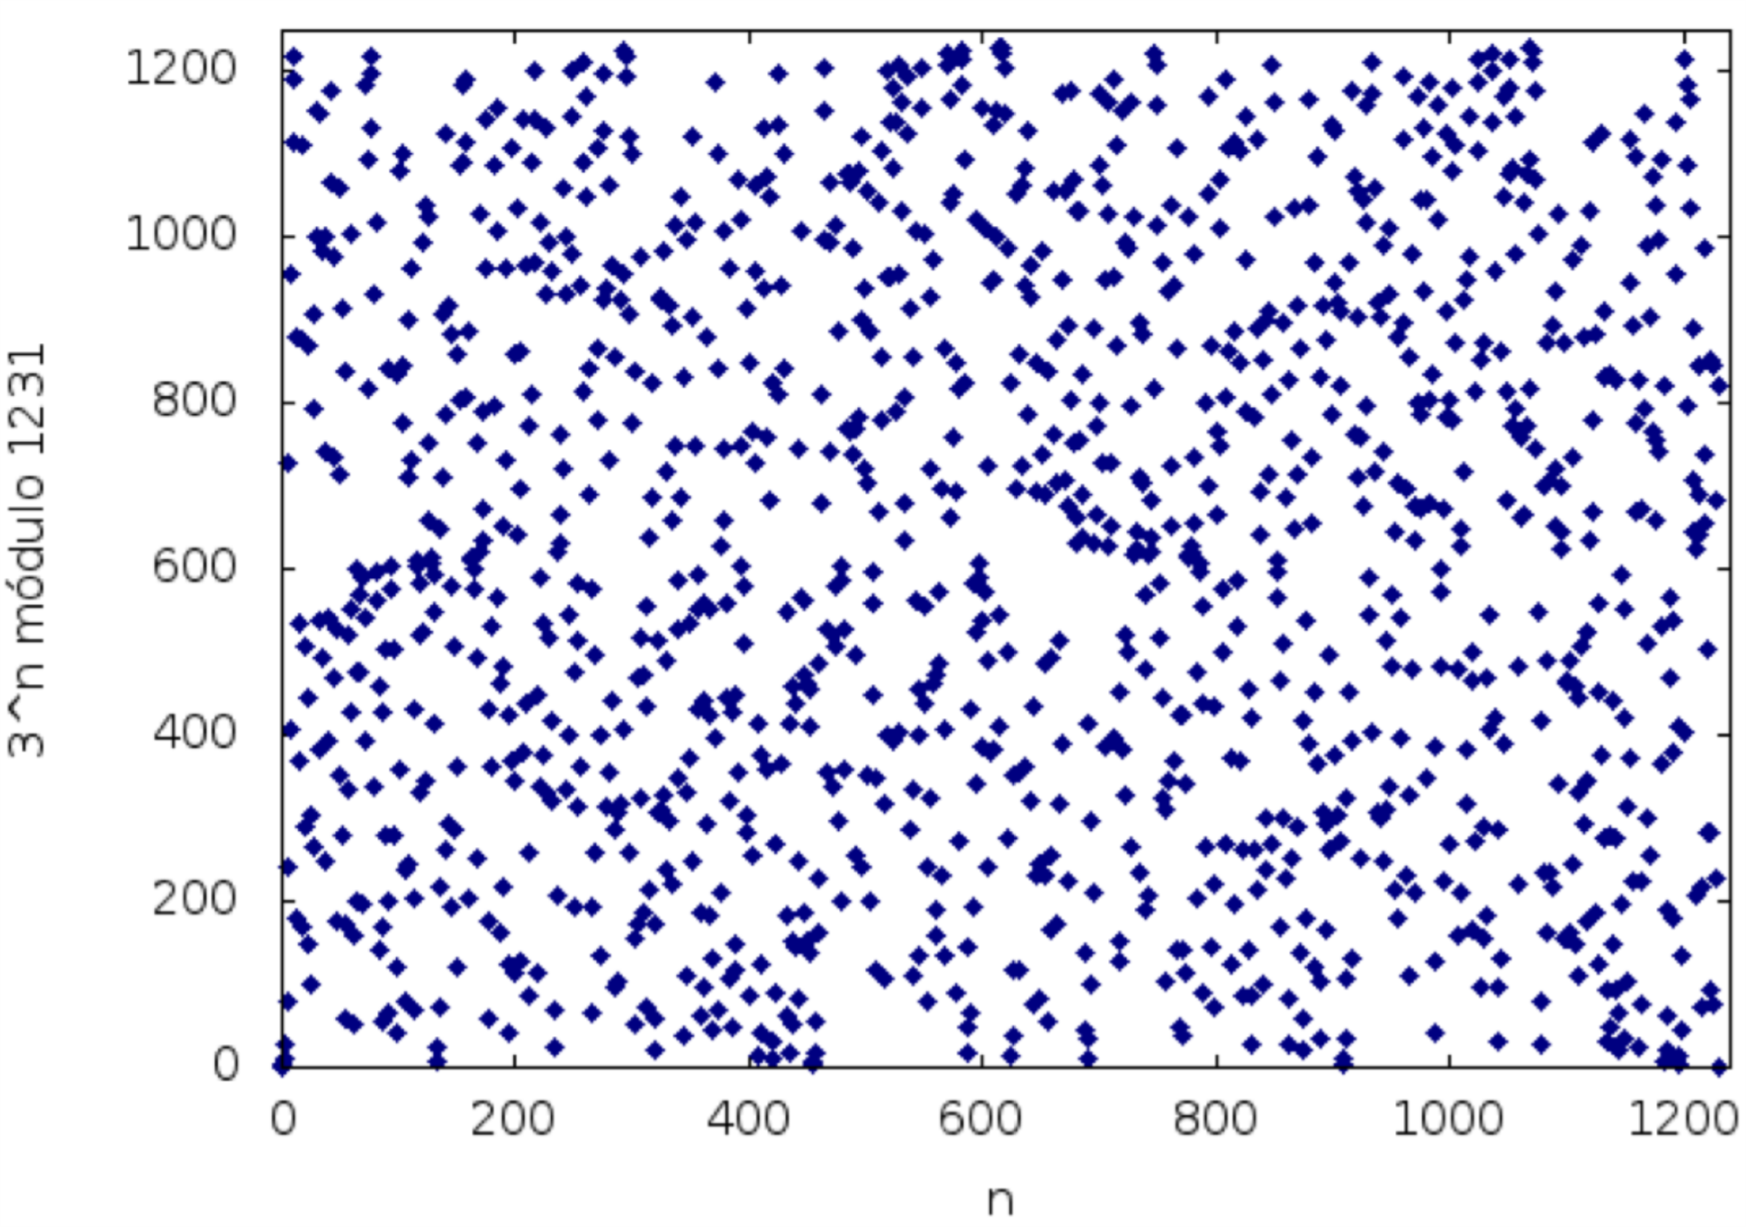
\includegraphics[width=\linewidth]{DL}
	\end{column}
	\begin{column}{0.5\textwidth}
		Discrete Logarithm with $G=\mathbb{Z}_{1231}$, $g=3$.
		
		\small{Adolfo Quirós Gracián. \textit{Grupos y criptografía: de Julio César a las curvas elípticas.}}
	\end{column}
	
\end{columns}
\end{frame}




\begin{frame}{Complexity classes}
\begin{block}{Definition (Polynomial-time reduction $L_1 \leq_P L_2$)}
Be $L_1$ and $L_2$ two decision problems. $L_1$ can be reduced in polynomial time to $L_2$ if $L_1$ can be solved using $L_2$ as a subroutine plus a polynomial time.
\end{block}

\begin{block}{Definition (Class NP-complete or NPC)}
A decision problems $L$ is in \textbf{NPC} if:
\begin{enumerate}
	\item $L \in $ \textbf{NP}, and
	\item $L_1 \leq_P L \quad \forall L_1 \in $ \textbf{NP}.
\end{enumerate}
\end{block}
\end{frame}



\begin{frame}{Hamiltonian Cycle \textsuperscript{NPC}}
\begin{description}[Parameters]
\item[Name] Hamiltonian Cycle Problem (HC).
\item[Parameters] Given graph $G=(V,E)$.
\item[Question] Does there exist a Hamiltonian cycle in $G$?
\end{description}

\begin{center}
\tikzstyle{every node}=[circle, draw, fill=black!50, inner sep=0pt, minimum width=8pt]
\begin{tikzpicture}[thick]
\draw [line width=0.8mm,purple](120:2) -- (240:2) -- (0:2) -- (0:0) -- cycle;
\draw (120:2) node {} -- (0:2) node {};
\draw (0:0) node {} -- (240:2) node {};
\end{tikzpicture}
\end{center}

\end{frame}


\begin{frame}{Graph 3-colorability \textsuperscript{NPC}}

\begin{description}[Parameters]
\item[Name] Graph 3-colorability Problem (G3C).
\item[Parameters] Given graph $G=(V,E)$.
\item[Question] Is there a function	$\phi : V \to \{1,2,3\}$ such that $\phi(u)\neq \phi(v) \quad \forall (u,v)\in E$?
\end{description}

\begin{center}
\begin{tikzpicture}[style=thick]
\draw (18:2cm) -- (90:2cm) -- (162:2cm) -- (234:2cm) --
(306:2cm) -- cycle;
\draw (18:1cm) -- (162:1cm) -- (306:1cm) -- (90:1cm) --
(234:1cm) -- cycle;
\foreach \x in {18,90,162,234,306}{
\draw (\x:1cm) -- (\x:2cm);
}
\draw (18:2cm) circle (5pt)[fill=blue!50];
\draw (90:2cm) circle (5pt)[fill=green!50];
\draw (162:2cm) circle (5pt)[fill=red!50];
\draw (234:2cm) circle (5pt)[fill=green!50];
\draw (306:2cm) circle (5pt)[fill=red!50];

\draw (18:1cm) circle (5pt)[fill=red!50];%4
\draw (162:1cm) circle (5pt)[fill=blue!50];%2
\draw (306:1cm) circle (5pt)[fill=green!50];%5
\draw (90:1cm) circle (5pt)[fill=red!50];%3
\draw (234:1cm) circle (5pt)[fill=blue!50];%1
\end{tikzpicture}
\end{center}

\end{frame}


\begin{frame}{Quadratic residue}
\begin{description}[Parameters]
\item[Name] Factorization problem (FACT).
\item[Parameters] Positive integer $N$.
\item[Question] Are there integers $p,q\geq 2$ such that $N = pq$?
\end{description}

\begin{description}[Parameters]
\item[Name] Quadratic residue problem (QR).
\item[Parameters] Given a composite integer $N=pq$ and the integer $x$ with Jacobi Symbol $\left( \frac{x}{N} \right) = 1$.
\item[Question] Is $x$ a quadratic residue in ${\mathbb Z}_N$? $\exists a\in {\mathbb Z}_N : x\equiv a^2 (N)$?
\end{description}

\begin{block}{Theorem}
$QR \leq_P FACT$
\end{block}

\end{frame}


















\begin{frame}{Residuos Cuadráticos: Símbolo de Jacobi}
\textbf{Propiedades} del S\'imbolo de Jacobi.

Sean $a,b \in {\mathbb Z}$ y sean $m$, $n$ enteros positivos impares:
\begin{enumerate}
	\item Si $a\equiv b~mod~n$ entonces $\left( \frac{a}{n} \right) = \left( \frac{b}{n} \right)$.
	\item $\left( \frac{a^2}{n} \right) = 1$.
	\item $\left( \frac{ab}{n} \right) = \left( \frac{a}{n} \right)\left( \frac{b}{n} \right)$.
	\item $\left( \frac{-1}{n} \right) = (-1)^{(n-1)/2}$.
	\item $\left( \frac{2}{n} \right) = (-1)^{(n^2-1)/8}$.
	\item $\left( \frac{m}{n} \right) = (-1)^{(n-1)(m-1)/4} \left( \frac{n}{m} \right)$ \textit{Ley de Reciprocidad Cuadr\'atica}.
\end{enumerate}
\end{frame}

\begin{frame}{Residuos Cuadráticos: Símbolo de Jacobi}
Podemos calcular el Símbolo de Jabobi $\left( \dfrac{a}{b} \right)$ en tiempo polinomial \textbf{sin conocer la factorización de} $b$: 
\begin{enumerate}
\item En caso de que $a$ sea mayor que $b$, reducirlo m\'odulo $b$, $a := a ~ mod ~b$.
\item Si $a$ es $0$, devolver $0$.
\item Si $a$ es $1$, devolver $1$.
\item Dividir $a$ por $2$ para ponerlo en la forma $a = 2^e a'$ con $a'$ impar. Si $e$ es par o $b \equiv \pm 1 ~mod~8$ poner $s := 1$, en caso contrario poner $s := -1$.
\item Finalmente si $a' \equiv 3 ~mod~4$ y $b \equiv 3~mod~4$ devolver $-s {\sf Jacobi}(b,a')$ y en caso contrario devolver $s {\sf Jacobi}(b,a')$.
\end{enumerate}
\end{frame}



\begin{frame}{Pruebas Interactivas}
\begin{definition}
	Denominamos clase de problemas \textbf{IP} (Interactivos en tiempo Polinomial) al conjunto de problemas de decisión para los que existe un sistema de prueba interactivo.
\end{definition}
\end{frame}



\begin{frame}{Pruebas Interactivas}
\begin{theorem}
\textbf{NP} $\subset$ \textbf{IP}.
\end{theorem}

\begin{proof}
Sea $Q$ un problema \textbf{NP}. Definimos el siguiente protocolo:
\begin{enumerate}
	\item  P resuelve la instancia del problema gracias a su capacidad de cómputo ilimitada y genera el certificado para V.
	\item  V recibe y verifica el certificado en tiempo polinomial. Si es válido, V acepta como $Verdadera$ la instancia. Si no, rechaza la prueba.
\end{enumerate}
%El protocolo es completo y robusto, con probabilidad nula de falso positivo, pues si la instancia es $Falsa$, ningún P puede generar un certificado que no existe.
\end{proof}
\end{frame}

\end{document}